% 
% PARTIE 2
% 
\section{Étude de la mobilité sur un sol plan \label{sec_2}}


\begin{obj}
L'objectif de cette partie est de valider les performances de mobilité, de manoeuvrabilité et
de contrôle du système de locomotion de ROBOVOLC. On cherche notamment à vérifier le
critère suivant du cahier des charges :

\begin{center}
\begin{tabular}{ll}
\hline
\textbf{Critère} & \textbf{Valeur} \\ \hline \hline
Vitesse de déplacement atteignable &   \SI{0,5}{m/s} \\\hline
\end{tabular}
\end{center}

\end{obj}



%%%%%%%
%%%%%%%     PARTIE  2.2
%\subsection{Présentation du système de locomotion}
%
%\begin{obj}
%Dans cette sous-partie, on présente l'architecture du système de locomotion de
%ROBOVOLC.
%\end{obj}
%
%
%La plateforme de ROBOVOLC est équipée d'un châssis et de six roues motrices indépendantes et
%non directionnelles réparties symétriquement sur trois essieux (\autoref{fig_04}).
%
%
%\begin{figure}[H]
%\centering
%\includegraphics[width=.45\linewidth]{fig_04.png}
%\caption{Schématisation de la plateforme de ROBOVOLC (vue de dessus) \label{fig_04}}
%\end{figure}
%
%
%Chaque roue représente un module autonome (\autoref{fig_05}) dont la chaîne d'énergie est constituée
%d'une batterie, d'un variateur de vitesse, d'un moteur électrique à courant continu, d'un réducteur
%de vitesse (de rapport de réduction $r=\dfrac{1}{236}$, entouré sur la \autoref{fig_05}), d'un capteur de vitesse et
%d'un micro-contrôleur.
%Les roues sont équipées de pneumatiques spéciaux de diamètre extérieur $D=\SI{300}{mm}$.
%
%
%
%\begin{figure}[H]
%\centering
%\includegraphics[width=.45\linewidth]{fig_05w.png}
%\caption{Schéma de transmission de puissance pour chaque roue (vue de dessus) \label{fig_05}}
%\end{figure}
%
%
%On introduit le nombre (adimensionnel) de Froude $Fr=\dfrac{v}{\sqrt{gl_c}}$
%qui caractérise la vitesse de
%déplacement $v$ de ROBOVOLC relativement à sa taille caractéristique $l_c$ ; $g$ est l'accélération de la
%pesanteur. Lorsque $Fr>1$, les effets dynamiques ont une influence importante sur la trajectoire.
%
%%Q2.1 :
%\question{Montrer que les effets dynamiques peuvent être ici négligés.}
%
%Dans la suite de cette partie, on suppose un roulement sans glissement longitudinal au niveau du
%contact roue-sol. On suppose de plus que le sol est plan et horizontal, que le contact roue-sol est
%ponctuel, et que le châssis et les roues sont des solides indéformables.
%
%\subsection{Comportement en ligne droite}
%
%\begin{obj}
%Dans cette sous-partie, on détermine la commande permettant d'assurer une vitesse de
%déplacement en ligne droite donnée.
%\end{obj}
%
%Une modélisation de la plateforme est donnée sur la \autoref{fig_06}. On définit un repère local
%$\repere{O}{x}{y}{z}$ lié au châssis, $\vect{x}$ correspondant à l'axe longitudinal du châssis (appelé aussi ligne de
%foi) illustré sur la \autoref{fig_04}, et $\vect{z} correspondant à l'axe vertical. Le point $O$ est le centre
%géométrique et de masse de la plateforme dans le plan $\left({O},\vect{x}\vect{y}\right)$ parallèle au sol.
%
%Pour chaque roue notée $S_i$ ( $1\leq i \leq 6$), on définit :
%\begin{itemize}
%\item le point de contact $P_i$ entre la roue et le sol ;
%\item le point $O_i$ qui est la projection du point $P_i$ sur l'axe de rotation de la roue.
%\end{itemize}
%
%
%La position de chaque point $O_i$ est définie par $\vect{OO_i}=a_i \vect{x}  +e_i\vect{y}$ avec $a_i=\pm a$ et $e_i=\pm e$.
%Le châssis est noté $S_c$ et le sol est noté $S_0$.

%%%%%%%
%%%%%%%     PARTIE  2.2 PAS FINIE DE RECOPIER !!!!!!



\subsection{Technologie et asservissement en vitesse}
Dans cette sous-partie, on étudie l'asservissement en vitesse des roues en analysant la
technologie des composants et en déterminant les propriétés de comportement.
Chacune des roues dispose d'une motorisation indépendante avec un asservissement en vitesse.
Le contrôle de la vitesse de rotation de chaque roue permet de minimiser le glissement
longitudinal, notamment en mode automatique lorsque ROBOVOLC doit suivre un cap de manière
autonome.
Le système d'asservissement qui équipe chaque roue est destiné à contrôler sa vitesse de rotation
et doit permettre au système embarqué de détecter un glissement (manque d'adhérence). Ce
système est modélisé sur la \autoref{fig_07}.


\begin{figure}[H]
\centering
\includegraphics[width=.45\linewidth]{fig_07.png}
\caption{Structure d'asservissement \label{fig_07}}
\end{figure}




La fonction $K_c$ représente un capteur de vitesse permettant de mesurer la vitesse de rotation du
moteur.


%Q2.9 :
\question{Citer deux composants permettant de réaliser la fonction $K_c$ en précisant les
avantages/inconvénients et le type de signal (analogique ou numérique) en entrée/sortie de
chacun. Indiquer, en justifiant, la technologie la plus probablement retenue ici.}

\subsubsection{Étude du convertisseur numérique-analogique (CNA)}

La valeur$U (t)$ en entrée du CNA est codée sous forme d'un entier non signé sur 16 bits. Elle est
ensuite convertie en grandeur analogique $\indice{U}{mot}$ entre $-\SI{10}{V}$ et $6\SI{10}{V}$ pour $U (t)$ évoluant en
hexadécimal de 0000 à sa valeur maximale FFFF.

%Q2.10 :
\question{Donner la valeur numérique de $U (t)$ à appliquer pour obtenir une valeur nulle en sortie
du CNA. A quelle consigne correspond la valeur hexadécimale d'entrée $U (t) =\text{A000}$?}

\subsubsection{Étude du convertisseur analogique-numérique (CAN)}

Le capteur utilisé pour mesurer la vitesse de rotation est de type dynamo-tachymétrique, ce choix
répondant aux exigences de tenue en température et robustesse. Le capteur fournit une tension
directement proportionnelle à la vitesse de rotation de la roue, cette tension variant au maximum
entre $-\SI{610}{mV}$ et $+\SI{650}{mV}$. Le CAN employé possède plusieurs canaux de conversion A/N 12 bits
d'une linéarité de +/-1 bit. Le temps de conversion par canal est de 25 micro-secondes.

%Q2.11 :
\question{Calculer la résolution en mV du CAN.}


%Q2.12 :
\question{Donner les deux hypothèses principales qu’il faut faire pour pouvoir utiliser un modèle de
système linéaire continu invariant.}

\subsubsection{Asservissement en vitesse}

On suppose dans la suite que :
\begin{itemize}
\item $C_v ( p)=K_v$ (constante) ;
\item $K_c =1$ (gain de capteur) ;
\item  les blocs CAN et CNA sont modélisés par des blocs unitaires.
\end{itemize}

La\autoref{fig_08} représente la réponse mesurée du moteur lorsqu’un échelon unitaire de tension est
envoyé en entrée.



%Q2.13 : 
\question{Exprimer par un modèle du premier ordre sous forme canonique la fonction de transfert
$\indice{H}{moteur}( p)$ du moteur, et identifier ses paramètres.}

%Q2.14 : 
\question{Calculer la fonction de transfert $\dfrac{\indice{\Omega}{roue}( p)}{\Omega_c(p)}$ sous forme canonique.}

%Q2.15 : 
\question{Exprimer les conditions pour avoir des valeurs d'erreur statique en position et en vitesse
inférieures à 1\%. Proposer un moyen d'obtenir ces erreurs statiques nulles.}


%% Partie 2.5 TODO
%\subsection{Maîtrise de trajectoire}









Les éruptions volcaniques peuvent avoir un impact important sur l'activité humaine, provoquant à
la fois des déplacements de population, des dégâts matériels, ainsi que des changements de
topographie et de climat. On considère qu'actuellement 10\% de la population terrestre vit sous la
menace des volcans, et 1500 volcans potentiellement en activité sont répertoriés sur la planète.
Par conséquent, une compréhension fine des phénomènes volcaniques et une meilleure maîtrise
des risques associés constituent un enjeu scientifique majeur.

Les observations scientifiques réalisées pendant les phases éruptives sont aujourd'hui
fondamentales pour l'étude des volcans. En effet, les prélèvements des gaz magmatiques et des
échantillons rocheux rejetés lors de ces phases constituent des indicateurs fiables de l'activité
interne des volcans ; ils sont donc une riche source d'informations pour les volcanologues.
Cependant, les phases éruptives sont aussi des phases actives très dangereuses et il est
primordial de limiter les risques humains lors d'observations et de prélèvements à proximité des
cratères en éruption (\autoref{fig_01}). 



\begin{figure}[H]
\centering
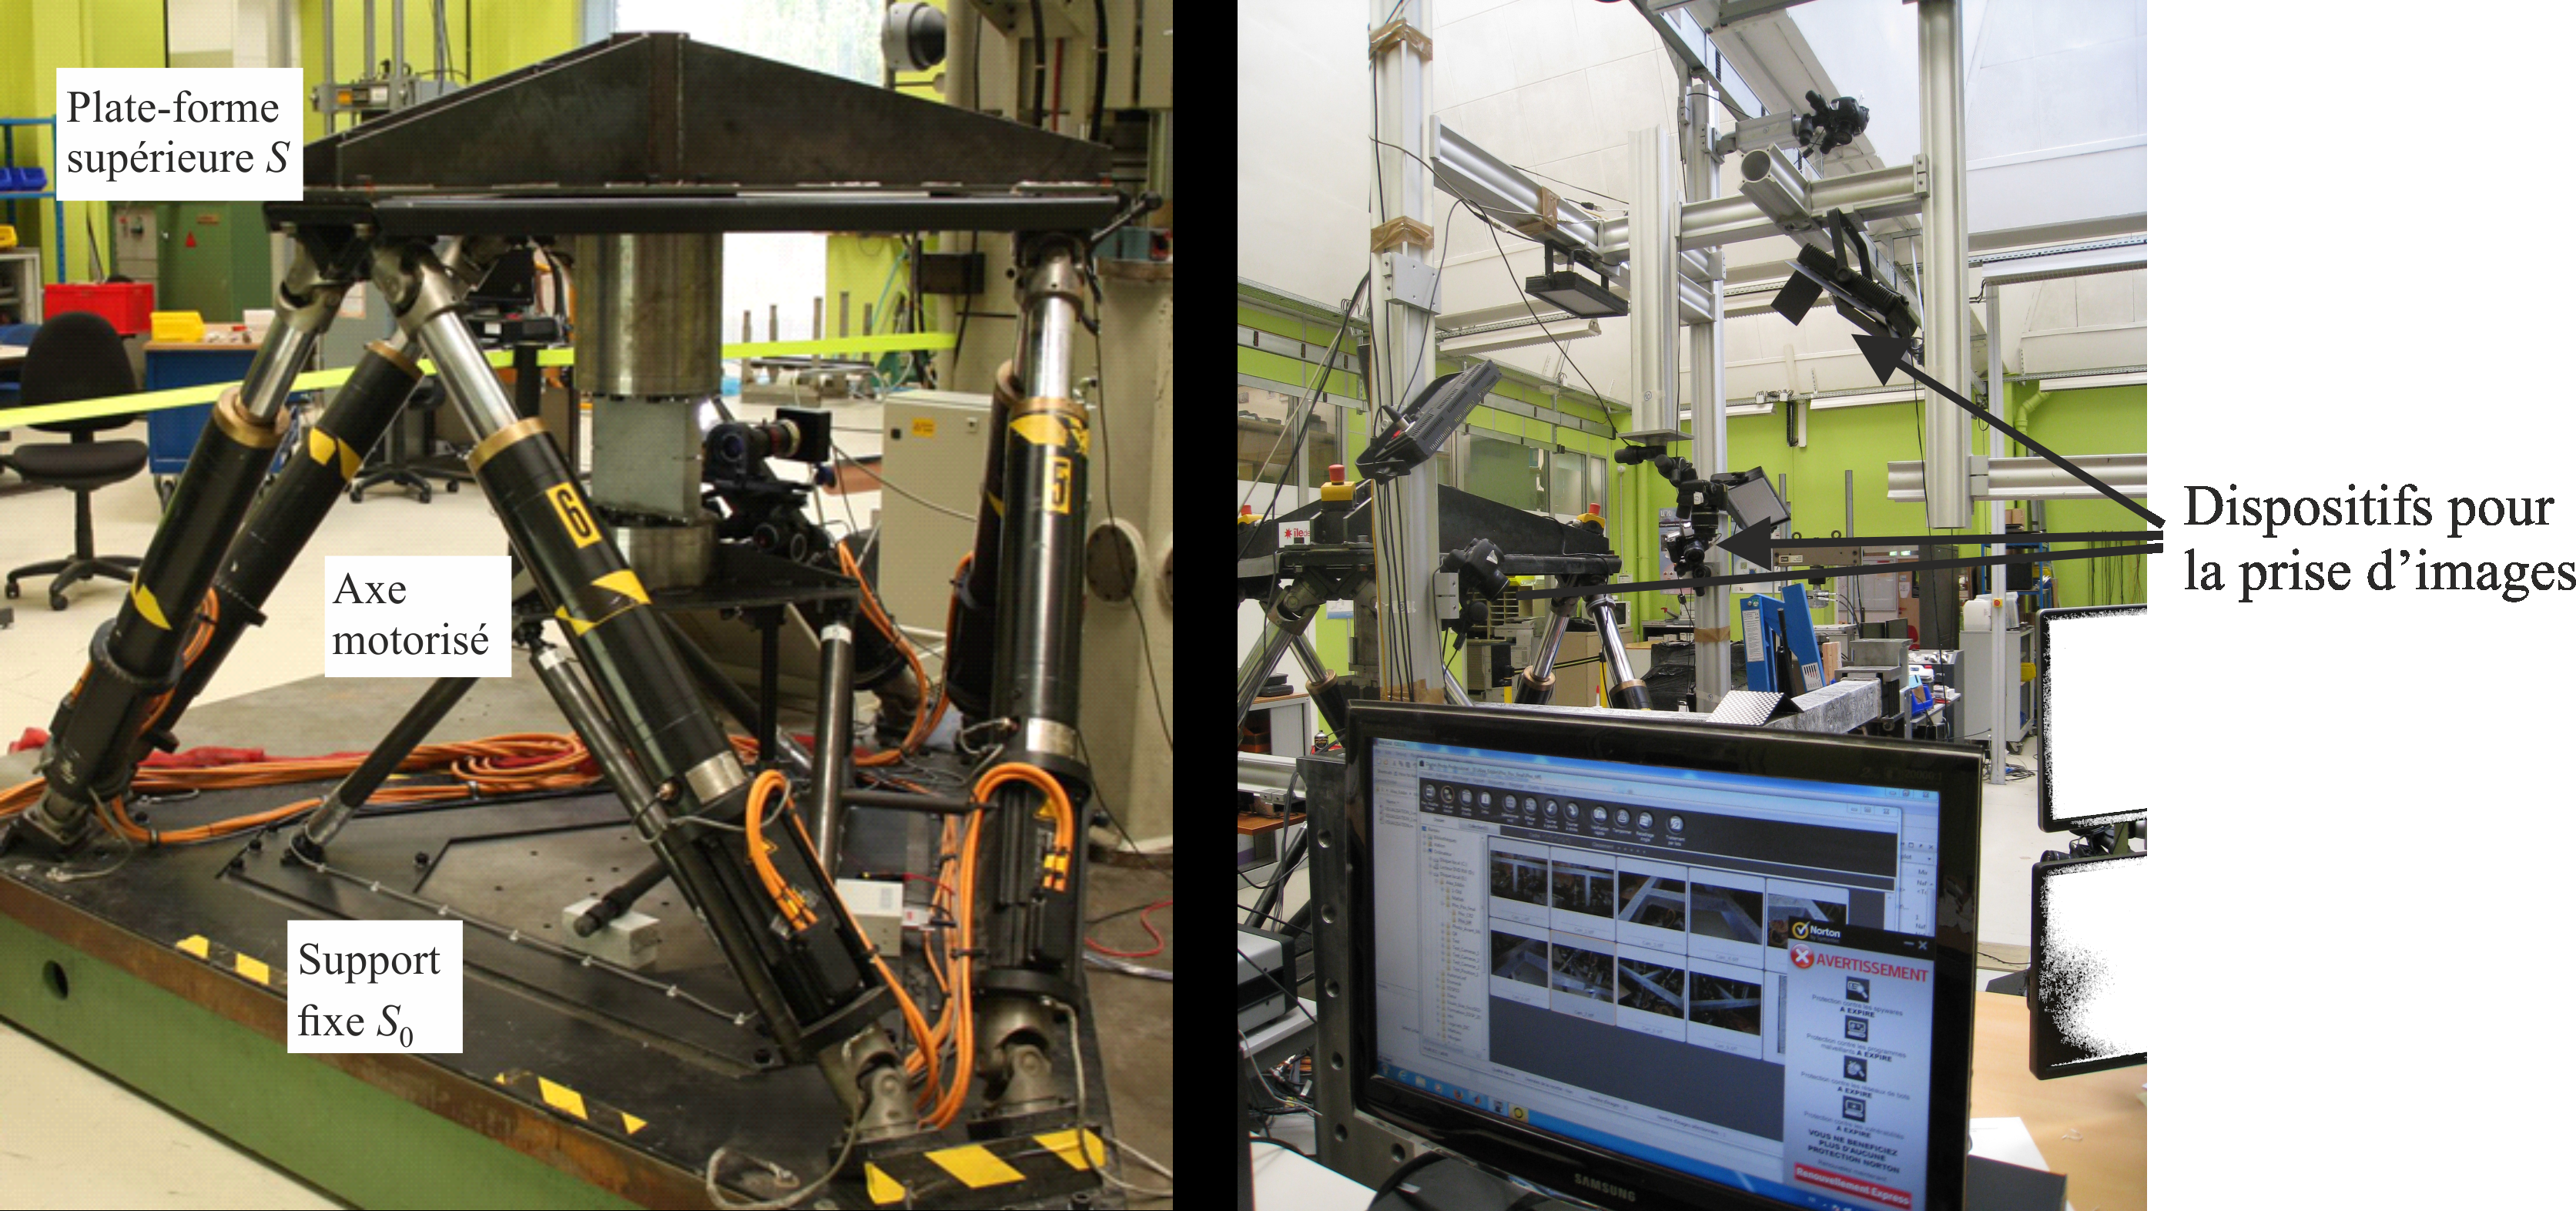
\includegraphics[width=.45\linewidth]{fig_01.png}
\caption{Schématisation d'un volcan en éruption \label{fig_01}}
\end{figure}


Avec ce constat, allié aux avancées technologiques dans le domaine de la robotique, la
Communauté Européenne a financé le projet ROBOVOLC dont le but était la réalisation d'un robot
mobile pour l'exploration volcanique. Ce robot devait être capable de :
\begin{itemize}
\item s'approcher d'un cratère actif ;
\item collecter des échantillons rocheux issus de rejets éruptifs ;
\item collecter des échantillons gazeux ;
\item collecter d'autres données physiques et chimiques.
\end{itemize}


\begin{obj}
Le sujet propose d'étudier quelques parties structurelles du système ROBOVOLC et de
valider plusieurs performances (liées à la mobilité et au prélèvement) de ce système. 
\end{obj}

\subsection{Présentation du système}


Le système ROBOVOLC est représenté sur la \autoref{fig_02}. Il se divise en plusieurs sous-systèmes
(liés à la navigation, au prélèvement et à la communication) qui sont détaillés dans les
diagrammes SysML fournis dans l'Annexe 1. 

\begin{figure}[H]
\centering
\includegraphics[width=.45\linewidth]{fig_02.png}
\caption{Représentation du système ROBOVOLC \label{fig_02}}
\end{figure}

La partie mécanique de ROBOVOLC est constituée de deux parties : (i) la plateforme (châssis,
roues) servant à la locomotion ; (ii) l'équipement d'analyse (bras manipulateur, pince, sondes) pour
le prélèvement et la mesure.

Une contrainte particulière dans la conception du système ROBOVOLC est qu'il est soumis à des
conditions extérieures particulièrement difficiles : terrain volcanique non structuré avec obstacles et
fortes pentes, températures très élevées près des zones éruptives (les gaz atteignent 600\degres C) mais
basses ailleurs à cause de l'altitude, présence de poussières de cendre très fines, ambiance
corrosive due aux composants acides, etc.


%Q1.1 : 
\question{Dans la phase de conception de ROBOVOLC, une alternative à un système de locomotion
à roues était un système volant. Donner deux inconvénients d'un tel système remettant en cause
son utilisation dans l'environnement volcanique considéré.}

ROBOVOLC est piloté à distance depuis un poste de contrôle (\autoref{fig_03}). La position géographique
du robot est obtenue par un système GPS et est envoyée au poste de contrôle par liaison radio.
De plus, l’opérateur peut visualiser en permanence les actions du système grâce aux images
transmises par une caméra embarquée.

L'énergie électrique nécessaire au système est apportée par une unité de puissance avec quatre
batteries couplées pour constituer deux unités de 24 V. La première est utilisée pour la plateforme,
l'autre pour l'équipement d'analyse. Ces batteries sont positionnées sur la partie basse du châssis.

%Q12
\question{Citer un intérêt à mettre les batteries en position basse sur le système.}


\begin{figure}[H]
\centering
\includegraphics[width=.45\linewidth]{fig_03.png}
\caption{Illustration du pilotage à distance du système ROBOVOLC\label{fig_03}}
\end{figure}

Un cahier des charges partiel est donné ci-dessous :

\begin{center}
\begin{tabular}{ll}
\hline
\textbf{Critère} & \textbf{Valeur} \\ \hline \hline
Distance maximale entre ROBOVOLC et le poste de contrôle & \SI{2}{km} \\ \hline  
Temps de trajet pour une mission de 24 heures 		& \SI{1,5}{h} \\ \hline 
Vitesse de déplacement atteignable 				& \SI{0,5}{m/s} \\ \hline 
Dimensions du système (longueur/largeur/hauteur) 		& \SI{1900}{mm} x \SI{1200}{mm}x \SI{800}{mm}\\ \hline 
Masse maximale des composants modulaires 			& \SI{200}{kg} \\ \hline 
Charge utile maximale (instruments, etc.) 			& \SI{30}{kg} \\ \hline 
Pente maximale du sol 						& 40\degres \\ \hline 
Hauteur maximale d'un obstacle 					& \SI{400}{mm} \\ \hline 
Diamètre des objets à saisir entre 				& \SI{40}{mm} et \SI{300}{mm} \\ \hline 
Masse maximale des objets à saisir 				& \SI{2,5}{kg} \\ \hline 
\end{tabular}
\end{center}



%Q1.3 : 
\question{Citer une phase de vie du système qui contraint sa taille maximale et son poids maximal.}

La suite du sujet est composée de quatre parties qui étudient quelques particularités de la
structure mécanique du système ROBOVOLC :
\begin{itemize}
\item les parties \ref{sec_2} et \ref{sec_3} étudient la phase de déplacement (roulage) du système : la partie \ref{sec_2} vise
à valider les performances de mobilité et de suivi de trajectoire du système sur un sol plan
tandis que la partie \ref{sec_3} vise à valider les performances de franchissement d'obstacle sur un
terrain accidenté ;
\item les parties \ref{sec_4} et \ref{sec_5} étudient la phase de préhension d'échantillon : la partie \ref{sec_4} vise à valider
les performances du bras manipulateur tandis que la partie \ref{sec_5} vise à valider les
performances de la pince.
\end{itemize}


